%%% Preamble
% Article class of KOMA-script with 11pt font and a4 format
\documentclass[paper=a4, fontsize=11pt]{scrartcl}	
\usepackage[T1]{fontenc}
\usepackage{fourier}

% English language/hyphenation
\usepackage[english]{babel}

% Better typography
\usepackage[protrusion=true,expansion=true]{microtype}

% Math packages
\usepackage{amsmath,amsfonts,amsthm}

% Enable pdflatex
\usepackage[pdftex]{graphicx}
\usepackage{url}

\usepackage{caption}
\usepackage{subcaption}

% Tables
\usepackage{multirow}

%%% Custom sectioning (sectsty package)
% Custom sectioning (see below)
\usepackage{sectsty}
% Change font of al section commands
\allsectionsfont{\centering \normalfont\scshape}

\setlength{\parindent}{25pt}

%%% Custom headers/footers (fancyhdr package)
\usepackage{fancyhdr}
\pagestyle{fancyplain}

% No page header
\fancyhead{}

% You may remove/edit this line 
\fancyfoot[L]{\small SIGB Hand-in 2}
\fancyfoot[C]{} % Empty
\fancyfoot[R]{\thepage} % Pagenumbering
\renewcommand{\headrulewidth}{0pt} % Remove header underlines
\renewcommand{\footrulewidth}{0pt} % Remove footer underlines
\setlength{\headheight}{13.6pt}


%%% Equation and float numbering
\numberwithin{equation}{section} % Equationnumbering: section.eq#
\numberwithin{figure}{section} % Figurenumbering: section.fig#
\numberwithin{table}{section} % Tablenumbering: section.tab#


%%% Maketitle metadata
\newcommand{\horrule}[1]{\rule{\linewidth}{#1}} % Horizontal rule

\title{
		%\vspace{-1in} 	
		\usefont{OT1}{bch}{b}{n}
		\normalfont \normalsize \textsc{IT University of Copenhagen} \\ [25pt]
		\horrule{0.5pt} \\[0.4cm]
		\huge Mandatory Assignment 2 \\
		\horrule{2pt} \\[0.5cm]
}

\author{
	\normalfont 
	\normalsize
	Miroslav Zoricak (mzor@itu.dk) \\[-3pt]
	\normalsize
	Arin Agha seyed hashem kadkhoda (aseh@itu.dk) \\[-3pt]
	\normalsize
	\today
}

\date{}


%%% Begin document
\begin{document}
\maketitle

\section{Introduction}

In this assignment we were tasked to explore various applications of homographies. Like the first assignment, to obtain our goal we used Python and OpenCV as a toolkit. The purpose is to learn how to use homographies because it’s related to both computer vision and computer graphics applications and is in general very useful for many applications. 

In this assignment we covered some used of homographies like point transfers, texture mapping, camera calibration and some of the benefits of having a calibrated camera, however we can’t cover all of the homographies uses because the time available for us is limited and there is extreme range of situation that homographies can be useful.



\section{Camera Calibration}
In this part we calibrated the camera and then loaded the calibration data that has been stored. Next we calculated the camera matrix for the first view of the calibration.
\begin{equation}
  P_{1} = K
	\begin{bmatrix} R_{1}|t_{1} \end{bmatrix}
\end{equation}
 After these steps we tried to check if P\textsubscript{1} is correct by projecting chesspattern points on the first camera view. As you can see in the \ref{fig:chesspattern} All the points have been projected exactly into the right position.
 
 \begin{figure}[h!]
	\centering
	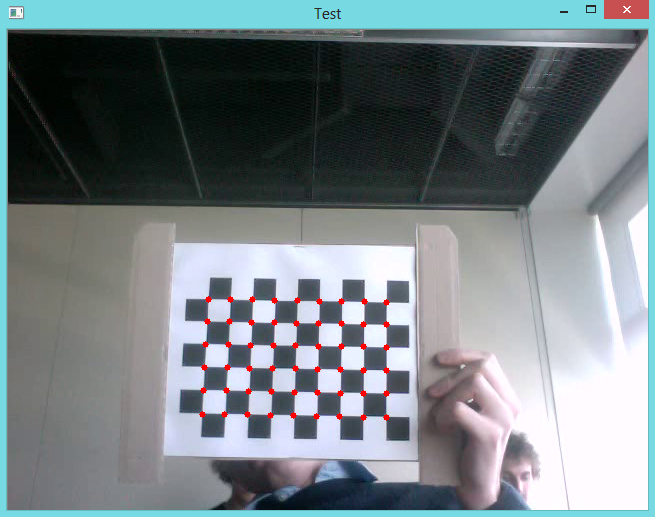
\includegraphics[width=\textwidth]{Handin3/images/patterndot.jpg}
	\caption{chesspattern}
	\label{fig:chesspattern}
\end{figure}
 
 In the last step of this part we tried to undistort the image by using the (cv2.undistort) function.(see figure \ref{eq:undistort})
 
 \begin{figure}[h!]
	\centering
	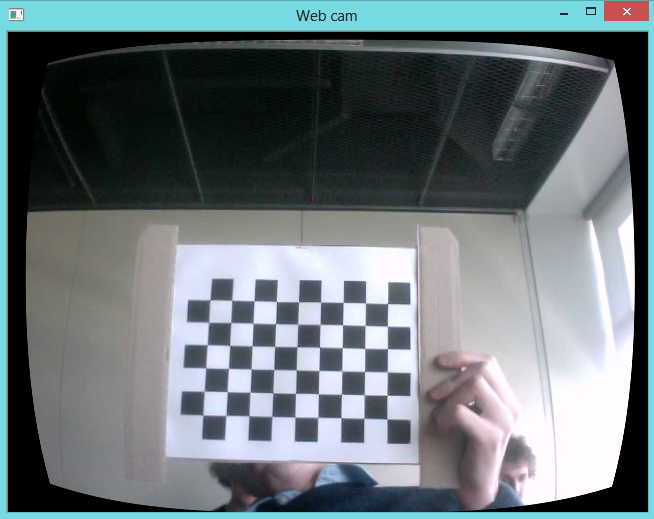
\includegraphics[width=\textwidth]{Handin3/images/undistort.jpg}
	\caption{undistort}
	\label{fig:undistort}
\end{figure}
 

\section{Augmented Cube}

\section{Back-face Culling and Texture Mapping}

To texture our wireframe model, we first calculate the homography between the texture (2D image) and a face of the cube as it is projected in the 2D final image. We then use this homography to perspective warp the texture into the final image. See Figure \ref{subfig:texture}. But this is obviously not right, some faces overlap others randomly. We solve this by a technique called back-face culling.

Back-face culling is a technique we've employed to address the problem that appears when we render the whole cube. In the 2D view you can not see all 5 textured faces of the cube at once. It is only possible to see one to three faces at any given time. Therefore some faces we render are redundant. All faces are drawn in the order in which the list containing their names is processed, so it is the same order always. Therefore the faces that are drawn later occlude faces drawn earlier, even though logically they should be behind them. 

To address this problem, a simple technique has been developed, where we determine the angle between the camera and a face, and based on that we decide whether or not to show the face. First we compute the unitary normal vector of the face. We take three points from the face, since we assume that the face is composed of four coplanar points, it does not matter which three we take, but the order does matter, because with wrong order we will get a normal that faces the other way (inside the cube). We then construct displacement vectors between two point pairs of the three points, and calculate the cross product of these vectors. As the last step we transform the obtained vector to get a unitary vector. 

Similarly we compute a vector from camera center and the center of the face we are comparing. We transform this vector to unitary as well. We can calculate the angle between the two vectors. If this angle is greater than 90 degrees, we know that the face is facing away from the camera, and we therefore don't draw it.

 \begin{figure}[h!]
	\begin{subfigure}[b]{0.5\textwidth}
		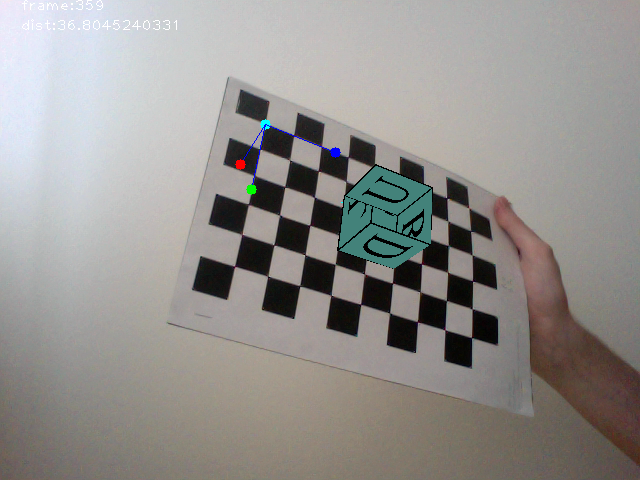
\includegraphics[width=\textwidth]{Handin3/images/culling.png}
		\caption{Texture Mapping}
		\label{subfig:texture}
	\end{subfigure}
	~
	\begin{subfigure}[b]{0.5\textwidth}
		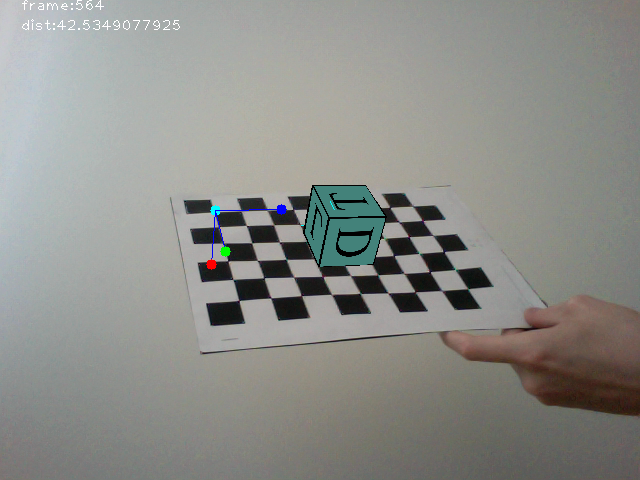
\includegraphics[width=\textwidth]{Handin3/images/texture2.png}
		\caption{Back-face Culling}
		\label{subfig:backculling}
	\end{subfigure}
	
	\label{fig:texturing}
	\caption{Backface Culling and Texture Mapping}
\end{figure}
\section{Conclusion}



%%% End document
\end{document}